% Options for packages loaded elsewhere
\PassOptionsToPackage{unicode}{hyperref}
\PassOptionsToPackage{hyphens}{url}
%
\documentclass[
]{book}
\usepackage{amsmath,amssymb}
\usepackage{lmodern}
\usepackage{iftex}
\ifPDFTeX
  \usepackage[T1]{fontenc}
  \usepackage[utf8]{inputenc}
  \usepackage{textcomp} % provide euro and other symbols
\else % if luatex or xetex
  \usepackage{unicode-math}
  \defaultfontfeatures{Scale=MatchLowercase}
  \defaultfontfeatures[\rmfamily]{Ligatures=TeX,Scale=1}
\fi
% Use upquote if available, for straight quotes in verbatim environments
\IfFileExists{upquote.sty}{\usepackage{upquote}}{}
\IfFileExists{microtype.sty}{% use microtype if available
  \usepackage[]{microtype}
  \UseMicrotypeSet[protrusion]{basicmath} % disable protrusion for tt fonts
}{}
\makeatletter
\@ifundefined{KOMAClassName}{% if non-KOMA class
  \IfFileExists{parskip.sty}{%
    \usepackage{parskip}
  }{% else
    \setlength{\parindent}{0pt}
    \setlength{\parskip}{6pt plus 2pt minus 1pt}}
}{% if KOMA class
  \KOMAoptions{parskip=half}}
\makeatother
\usepackage{xcolor}
\usepackage{color}
\usepackage{fancyvrb}
\newcommand{\VerbBar}{|}
\newcommand{\VERB}{\Verb[commandchars=\\\{\}]}
\DefineVerbatimEnvironment{Highlighting}{Verbatim}{commandchars=\\\{\}}
% Add ',fontsize=\small' for more characters per line
\usepackage{framed}
\definecolor{shadecolor}{RGB}{248,248,248}
\newenvironment{Shaded}{\begin{snugshade}}{\end{snugshade}}
\newcommand{\AlertTok}[1]{\textcolor[rgb]{0.94,0.16,0.16}{#1}}
\newcommand{\AnnotationTok}[1]{\textcolor[rgb]{0.56,0.35,0.01}{\textbf{\textit{#1}}}}
\newcommand{\AttributeTok}[1]{\textcolor[rgb]{0.77,0.63,0.00}{#1}}
\newcommand{\BaseNTok}[1]{\textcolor[rgb]{0.00,0.00,0.81}{#1}}
\newcommand{\BuiltInTok}[1]{#1}
\newcommand{\CharTok}[1]{\textcolor[rgb]{0.31,0.60,0.02}{#1}}
\newcommand{\CommentTok}[1]{\textcolor[rgb]{0.56,0.35,0.01}{\textit{#1}}}
\newcommand{\CommentVarTok}[1]{\textcolor[rgb]{0.56,0.35,0.01}{\textbf{\textit{#1}}}}
\newcommand{\ConstantTok}[1]{\textcolor[rgb]{0.00,0.00,0.00}{#1}}
\newcommand{\ControlFlowTok}[1]{\textcolor[rgb]{0.13,0.29,0.53}{\textbf{#1}}}
\newcommand{\DataTypeTok}[1]{\textcolor[rgb]{0.13,0.29,0.53}{#1}}
\newcommand{\DecValTok}[1]{\textcolor[rgb]{0.00,0.00,0.81}{#1}}
\newcommand{\DocumentationTok}[1]{\textcolor[rgb]{0.56,0.35,0.01}{\textbf{\textit{#1}}}}
\newcommand{\ErrorTok}[1]{\textcolor[rgb]{0.64,0.00,0.00}{\textbf{#1}}}
\newcommand{\ExtensionTok}[1]{#1}
\newcommand{\FloatTok}[1]{\textcolor[rgb]{0.00,0.00,0.81}{#1}}
\newcommand{\FunctionTok}[1]{\textcolor[rgb]{0.00,0.00,0.00}{#1}}
\newcommand{\ImportTok}[1]{#1}
\newcommand{\InformationTok}[1]{\textcolor[rgb]{0.56,0.35,0.01}{\textbf{\textit{#1}}}}
\newcommand{\KeywordTok}[1]{\textcolor[rgb]{0.13,0.29,0.53}{\textbf{#1}}}
\newcommand{\NormalTok}[1]{#1}
\newcommand{\OperatorTok}[1]{\textcolor[rgb]{0.81,0.36,0.00}{\textbf{#1}}}
\newcommand{\OtherTok}[1]{\textcolor[rgb]{0.56,0.35,0.01}{#1}}
\newcommand{\PreprocessorTok}[1]{\textcolor[rgb]{0.56,0.35,0.01}{\textit{#1}}}
\newcommand{\RegionMarkerTok}[1]{#1}
\newcommand{\SpecialCharTok}[1]{\textcolor[rgb]{0.00,0.00,0.00}{#1}}
\newcommand{\SpecialStringTok}[1]{\textcolor[rgb]{0.31,0.60,0.02}{#1}}
\newcommand{\StringTok}[1]{\textcolor[rgb]{0.31,0.60,0.02}{#1}}
\newcommand{\VariableTok}[1]{\textcolor[rgb]{0.00,0.00,0.00}{#1}}
\newcommand{\VerbatimStringTok}[1]{\textcolor[rgb]{0.31,0.60,0.02}{#1}}
\newcommand{\WarningTok}[1]{\textcolor[rgb]{0.56,0.35,0.01}{\textbf{\textit{#1}}}}
\usepackage{longtable,booktabs,array}
\usepackage{calc} % for calculating minipage widths
% Correct order of tables after \paragraph or \subparagraph
\usepackage{etoolbox}
\makeatletter
\patchcmd\longtable{\par}{\if@noskipsec\mbox{}\fi\par}{}{}
\makeatother
% Allow footnotes in longtable head/foot
\IfFileExists{footnotehyper.sty}{\usepackage{footnotehyper}}{\usepackage{footnote}}
\makesavenoteenv{longtable}
\usepackage{graphicx}
\makeatletter
\def\maxwidth{\ifdim\Gin@nat@width>\linewidth\linewidth\else\Gin@nat@width\fi}
\def\maxheight{\ifdim\Gin@nat@height>\textheight\textheight\else\Gin@nat@height\fi}
\makeatother
% Scale images if necessary, so that they will not overflow the page
% margins by default, and it is still possible to overwrite the defaults
% using explicit options in \includegraphics[width, height, ...]{}
\setkeys{Gin}{width=\maxwidth,height=\maxheight,keepaspectratio}
% Set default figure placement to htbp
\makeatletter
\def\fps@figure{htbp}
\makeatother
\setlength{\emergencystretch}{3em} % prevent overfull lines
\providecommand{\tightlist}{%
  \setlength{\itemsep}{0pt}\setlength{\parskip}{0pt}}
\setcounter{secnumdepth}{5}
\usepackage{booktabs}
\usepackage{amsthm, graphicx, mathtools, amssymb, amsmath}
\makeatletter
\def\thm@space@setup{%
  \thm@preskip=8pt plus 2pt minus 4pt
  \thm@postskip=\thm@preskip
}
\makeatother

\newtheorem*{adamCitation}{Citation}
\newtheorem*{remark}{Remark}
\newtheorem*{definition}{Definition}
\newtheorem*{task}{Task}
\newtheorem*{solution}{Solution}
\DeclareMathOperator\Arg{Arg}
\usepackage{booktabs}
\usepackage{longtable}
\usepackage{array}
\usepackage{multirow}
\usepackage{wrapfig}
\usepackage{float}
\usepackage{colortbl}
\usepackage{pdflscape}
\usepackage{tabu}
\usepackage{threeparttable}
\usepackage{threeparttablex}
\usepackage[normalem]{ulem}
\usepackage{makecell}
\usepackage{xcolor}
\ifLuaTeX
  \usepackage{selnolig}  % disable illegal ligatures
\fi
\usepackage[]{natbib}
\bibliographystyle{elsarticle-harv}
\IfFileExists{bookmark.sty}{\usepackage{bookmark}}{\usepackage{hyperref}}
\IfFileExists{xurl.sty}{\usepackage{xurl}}{} % add URL line breaks if available
\urlstyle{same} % disable monospaced font for URLs
\hypersetup{
  pdftitle={Time Series Analysis and Forecasting with Complex Dynamic Models},
  pdfauthor={Sergey Svetunkov and Ivan Svetunkov},
  hidelinks,
  pdfcreator={LaTeX via pandoc}}

\title{Time Series Analysis and Forecasting with Complex Dynamic Models}
\author{Sergey Svetunkov and Ivan Svetunkov}
\date{2022-11-06}

\begin{document}
\maketitle

{
\setcounter{tocdepth}{1}
\tableofcontents
}
\hypertarget{introduction}{%
\chapter*{Introduction}\label{introduction}}
\addcontentsline{toc}{chapter}{Introduction}

The theory of complex variables functions is actively used in a variety of disciplines, including modern physics and engineering sciences. It is relatively easy to describe the complex phenomena that are studied in these areas of science using the models and methods of this branch of mathematics. Social sciences, being much more complicated due to the unpredictability of human behaviour, tend to use simpler instruments for modelling complex processes (references). For example, there are only few scientific publications in which methods and models of the theory of complex variables functions are used in economics, and they typically use that instrument for diagnostics or statistical tests (references) rather than proper modelling.

In 2012, Springer published the monograph ``Complex-valued Modeling in Economics and Finance'' (Svetunkov, 2012), which presented the theory and methodology of modelling using complex variables in economics. Svetunkov (2012) have summarised the main principles of using complex variables in economics and discussed how to estimate some of those models. While, this was the first monograph that discussed the topic, the first paper in this direction was Ben Tamari (1997). The author first introduced Wealth as a complex variable consisting of Output (real part) and Money (imaginary part) and showed how, even with such an elementary representation, interesting new results can be obtained in the area of economics. Unfortunately, this work has gone unnoticed in scientific world. We became aware of this work only in 2016, when Ben Tamari had kindly sent Sergey Svetunkov his paper.

Since 2012, there has been some development in the area of modelling using complex variables, notably a paper by Svetunkov \& Kourentzes (2022) on Complex Exponential Smoothing and Kourentez et al.~(2019) on an error measure based on the idea of complex numbers. Up until now, the modelling with complex variables has been mainly picked up by academics working in the areas of forecasting and engineering. The latter group has been using complex autoregressions for a couple of decades, modelling and predicting signals. The former group has only started using the principles described in Svetunkov (2012). In other disciplines, complex variables are not used directly for model building. The probable reason for this is the lack of the communication between the disciplines and the inherited inertia of academia.

In a try to speed up the adoption of the new instrument, we have written this monograph, summarising the research that has been done in the area of dynamic models since 2012. We should clarify that the term ``dynamic model'' used in this monograph refers to models that have a structure that changes over time. The classical example of such a model is ARIMA (AutoRegression Integrated with Moving Average by Box \& Jenkins, 1976), which allows producing forecasts for a variety of processes based on the existing historical time series. Another example is a multivariate version of ARMA, Vector ARMA or VARMA, which allows modelling the dynamics of several related processes simultaneously. For instance, in business and economics, these models are used for prices, demand forecasting and for capturing complex interactions between macroeconomic indicators over time.
However, all autoregression models that exist today use real variables. In this monograph we will discuss their complex-valued counterparts, namely complex ARIMA and complex VARMA, and study their properties, showing how to identify their orders and how to estimate these models in practice. But before rushing into the discussion, we will explain the basics of random complex variables and complex-valued statistics, which has been developed in signal processing literature, but has not been used to its full potential.

Chapter 1 discusses the theory of random complex variables, conventional and complex-valued statistics, the complex least squares method, maximum likelihood and complex autocorrelation and partial autocorrelation functions. In Chapter 2, we will move to the discussion of simple dynamic model -- complex AR, starting from its properties and slowly moving to its identification and estimation and then to forecasting. After that, in Chapter 3, we will move towards complex MA, again discussing its properties and how one can apply it in practice. The two parts will be united in a cARIMA model in Chapter 4, where we will also discuss seasonal counterpart of the model. Finally, we will move to vector models in Chapter 5, introducing cVAR, cVMA and cVARMA, showing their advantages in comparison with the conventional real valued models. All of this will be supported by examples in R, which will rely heavily on the package ``complex'', developed especially for this monograph. This means that anyone can then use the proposed models for purposes of time series analysis and forecasting.
This work was partially supported by the Russian Foundation for Basic Research (grant No.~19-010-00610\textbackslash19 ``Theory, methods and methodologies of forecasting economic development by autoregression models of complex variables''). Thanks to this support, it became possible to carry out this research in general, forming a new scientific direction in statistical modelling and short-term forecasting.

The authors are grateful to those young scientists of St.~Petersburg Polytechnic University of Peter the Great, who participated in this study, patiently testing the author's hypotheses. They helped forming the theory behind the models discussed in this monograph. We are pleased to mention their names: Evgeny Goltsev, Nikolai Pitukhin, Victoria Matskevich, Yulia Selivanova, Galina Siruk and Nazira Shaikhleeva.

this monograph relies heavily on the \texttt{complex} package for R. Many of the examples in R will use functions from this package, so make sure to install it before running any R code \citep{R-complex}:

\begin{Shaded}
\begin{Highlighting}[]
\FunctionTok{install.packages}\NormalTok{(}\StringTok{"complex"}\NormalTok{)}
\end{Highlighting}
\end{Shaded}

\hypertarget{intro}{%
\chapter{Introduction to random complex variables}\label{intro}}

\hypertarget{theory-of-complex-variables}{%
\section{Theory of complex variables}\label{theory-of-complex-variables}}

This section sets out the basic concepts of the Theory of Complex Variables Functions (TCVF) with some historical overlook of the idea of complex numbers. Hopefully, this will help in understanding the main idea that we will use extensively in the following chapters.

The theory of complex numbers started in 1572 in the small Italian town of Kura. It was in this place and precisely in this year that the manuscript of an Italian mathematician Rafael Bombelli was published. The book was called Algebra. Rafael Bombelli showed in it how to solve the following cubic equation:
\begin{equation}
    x^3 = 15x + 4 .
    \label{eq:BombelliEquation}
\end{equation}
The root of cubic equations at that time was calculated using the formula of Scipione del Ferro. With regards to the task at hand, finding the root should have been carried out as follows:
\begin{equation}
    \begin{aligned}
    x = & \sqrt[3]{\frac{4}{2}+\sqrt{\left(\frac{4}{2}\right)^2 - \left(\frac{15}{3}\right)^3}} + \sqrt[3]{\frac{4}{2}-\sqrt{\left(\frac{4}{2}\right)^2 - \left(\frac{15}{3}\right)^3}} = \\
        & \sqrt[3]{2+\sqrt{-121}} + \sqrt[3]{2-\sqrt{-121}} .
    \end{aligned}
    \label{eq:BombelliSolution}
\end{equation}
As can be seen from equation \eqref{eq:BombelliSolution}, there are several square roots, and it follows directly from the right hand side of this equation that to calculate the roots of equation \eqref{eq:BombelliEquation}, we need to extract the square root from the negative number, -121. This means that it will not be possible to find a solution to this equation in the domain of real numbers.

This does not mean that equation \eqref{eq:BombelliEquation} does not have a solution. If you represent the problem graphically on a plane then it is easy to see that there is one. But it is impossible to find it arithmetically using the Scipione del Ferro formula, because there is a negative number in the expression on the right-hand side of \eqref{eq:BombelliSolution}, and back then, mathematicians were sure that the square root of a negative number does not exist.

The mathematicians of that time struggled to solve this problem, and Rafael Bombelli suggested to ignore the negative sign in the expression (Bombelli, 12). After all, the number -121 can be represented as a product of two numbers: -1 and 121. Then the square root of this number can be written as \(\sqrt{-1} \times 11\). So, formula \eqref{eq:BombelliSolution} becomes:
\begin{equation}
    x = \sqrt[3]{2+11\sqrt{-1}} + \sqrt[3]{2-11\sqrt{-1}} .
    \label{eq:BombelliSolutionSqrt}
\end{equation}
Now it is possible to get a solution of the problem, and the root of the cubic equation is \(x = 4\).

For a long time, Bombelli's approach was considered by scientists as a convenient mathematical trick. And the square root of minus one was called ``magic unit'', ``vanishing unit'', etc. Finally, the term ``imaginary unit'' was established by René Descartes in 1637 and any number multiplied by the imaginary unit would be called ``imaginary number''. Merging a real number with an imaginary number gives another number, which can be considered as a more general to the two, which is called ``complex''. It can be written as:
\begin{equation}
    z = x+iy ,
    \label{eq:complexNumber}
\end{equation}
where \(x\) is the real part, \(iy\) is the imaginary part of a complex number, \(x\) and \(y\) are real numbers and \(i\) is the imaginary unit that satisfies the equality:
\begin{equation}
    i^2 = -1 .
    \label{eq:imaginaryUnit}
\end{equation}

With complex numbers, one can perform almost all the same operations as with the real ones. However, taking into account the properties of the imaginary unit, these operations can lead to results that are not common in the domain of real numbers.

The main problem that analysts face when trying to understand a complex number is the complexity of the interpretation of the imaginary part. The main question in this case can be formulated as: Where do imaginary numbers appear in practice? And what is the practical meaning of an imaginary unit? We have heard questions like that many times, and while they are valid, we think that they do not have appropriate answers and divert the analysts from what the modelling with complex variables brings.

We argue that the imaginary unit does not have any practical meaning: neither in economics, nor in sociology, nor in engineering, nor in physics. The imaginary unit is a mathematical rule, and that is all. It is a mathematical abstract that has useful properties. A number \(\sqrt{2}\) or \(\ln 3\) do not have practical meaning either, but they are useful for modelling purposes and solving applied problems in a variety of disciplines. Similarly, an imaginary unit is convenient for solving a whole class of problems in different areas of application. With the help of the rules specified by conditions \eqref{eq:complexNumber} and \eqref{eq:imaginaryUnit}, it is possible to use new mathematical operations, obtain new mathematical results, and create new mathematical models.

Imaginary and complex numbers are mathematical instruments that can help in describing a real-life phenomenon. If a researcher decides to use complex variables for real processes modelling, they will need to predefine the rules according to which one component of a complex process is attributed to the real part, and another one is attributed to the imaginary part of the complex variable. These rules might seem arbitrary, because there is no ``true'' recipe, according to which the assignment to complex variable parts should be done. The main motivation for them is the efficiency of modelling (such as goodness of fit or forecasting accuracy) and nothing else.

In order to better understand how the modelling with complex variables can be done, we need to better understand how complex variables can be represented and interpreted. A real number represents visually a certain segment on the numerical axis, which has a zero point and a multitude of values from minus infinity to infinity. Any real number is characterized by the distance from zero to the value of that number. Negative numbers are located to the left of zero, while the positive ones are located to the right of it.

A complex number consists of two parts, which can be visualised on the plane with two perpendicular axes, where the real numbers are marked on the horizontal line, and the imaginary ones are on the vertical one. This is shown visually in Figure \ref{fig:complexPlane} with a complex number \(z=x+iy\).

\begin{figure}
\centering
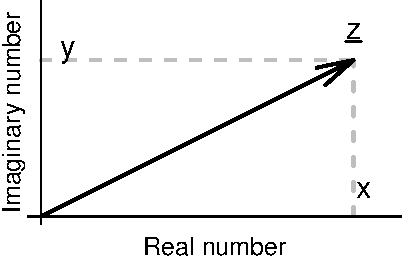
\includegraphics{Svetunkov---Svetunkov---Complex-Dynamic-Models_files/figure-latex/complexPlane-1.pdf}
\caption{\label{fig:complexPlane}Visual presentation of a complex number on the complex plane.}
\end{figure}

Any point lying on the complex plane in Figure \ref{fig:complexPlane} characterises a complex number, even if that point lies on the axis of real numbers. In that specific case, we would be talking about a complex number with a zero imaginary part, i.e.~\(z=x+i0\).

Given that complex numbers can be represented on a plane (in so called Cartesian coordinates), the number \eqref{eq:complexNumber} can be represented in a form of a vector that starts in the origin of coordinates and ends at the point (x, y). Then any complex number can be represented in form of polar coordinates using the magnitude of the vector and its polar angle:
\begin{equation}
    z = x+iy = r (\cos \phi + i \sin \phi),
    \label{eq:complexNumberTrigonometric}
\end{equation}
where \(r=|z|\) is the magnitude, which is calculated as a Euclidean distance from the origin to the point (x, y) on the plane:
\begin{equation}
    r = \sqrt{x^2 + y^2},
    \label{eq:complexNumberMagnitude}
\end{equation}
and \(\phi=\Arg(z)\) is the angle, which equals to:
\begin{equation}
    \phi = \arctan \frac{y}{x} + 2 \pi l,
    \label{eq:complexNumberAngle}
\end{equation}
where \(l\) is an integer number. While depending on a task, \(l\) can be set to a positive, a negative number, or a zero, for convenience, we will restrict it to \(l=0\), because all the other values will not be useful for the inference in following chapters. The polar angle is sometimes referred to as the argument of a complex number.

Using the magnitude and the polar angle, we can also represent any complex number in the exponential form (which was first proposed by Euler):
\begin{equation}
    z = r e^{i \phi} ,
    \label{eq:complexNumberExponential}
\end{equation}
where \(e\) is the Euler's constant. In this form, the positive real number has \(\phi=0\), while the negative one has \(\phi=\pi\), and all imaginary numbers have an angle dividable by \(\frac{\pi}{2}\). So, for example:
\begin{equation*}
    \begin{aligned}
    41 = & 41 e^{i 0} \\
    i41 = & 41 e^{i \frac{\pi}{2}} \\
    -41 = & 41 e^{i \pi} \\
    -i41 = & 41 e^{i \frac{3 \pi}{2}}
    \end{aligned}
\end{equation*}
The multiplication of any complex number by the imaginary unit in this case implies the rotation by \(\frac{\pi}{2}\), as shown in Figure \ref{fig:complexPlaneMultiplication}, where a complex variable \(z_1 = x_1 + i y_1\) becomes \(z_2 = z_1 \times i = x_2 + i y_2\) etc.

\begin{figure}
\centering
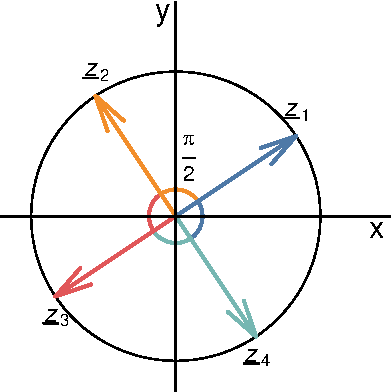
\includegraphics{Svetunkov---Svetunkov---Complex-Dynamic-Models_files/figure-latex/complexPlaneMultiplication-1.pdf}
\caption{\label{fig:complexPlaneMultiplication}Multiplication of a complex number by \(i\) implies the rotation of it by \(\frac{\pi}{2}\).}
\end{figure}

In a way, any mathematical operation with a complex number implies a change in magnitude and angle of the number, while the multiplication and division by a number with non-zero imaginary part will always lead to the rotation of the number.

Furthermore, given that any complex number can be represented in the exponential form, it can also be visualised on a polar coordinates plane, where the magnitude is marked on the x-axis, and the polar angle is marked on the y-axis. This is shown visually in Figure \ref{fig:complexPlanePolar}.

\begin{figure}
\centering
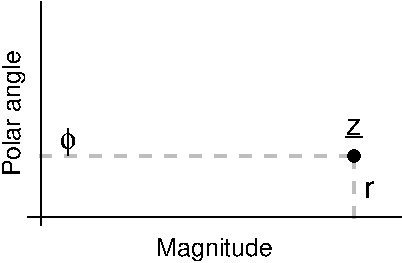
\includegraphics{Svetunkov---Svetunkov---Complex-Dynamic-Models_files/figure-latex/complexPlanePolar-1.pdf}
\caption{\label{fig:complexPlanePolar}Visual presentation of a complex number in the polar coordinates.}
\end{figure}

The usefulness of the polar coordinates presentation becomes apparent when a set of complex numbers is considered, because then in some cases it becomes possible to see some relations that were not obvious on the Cartesian plane. Figure \ref{fig:complexCartesianvsPolar} shows an example of a complex random variable, for which the real and imaginary parts do not seem to have any obvious linear relation, but the magnitude and the angle have a negative relation.

\begin{figure}
\centering
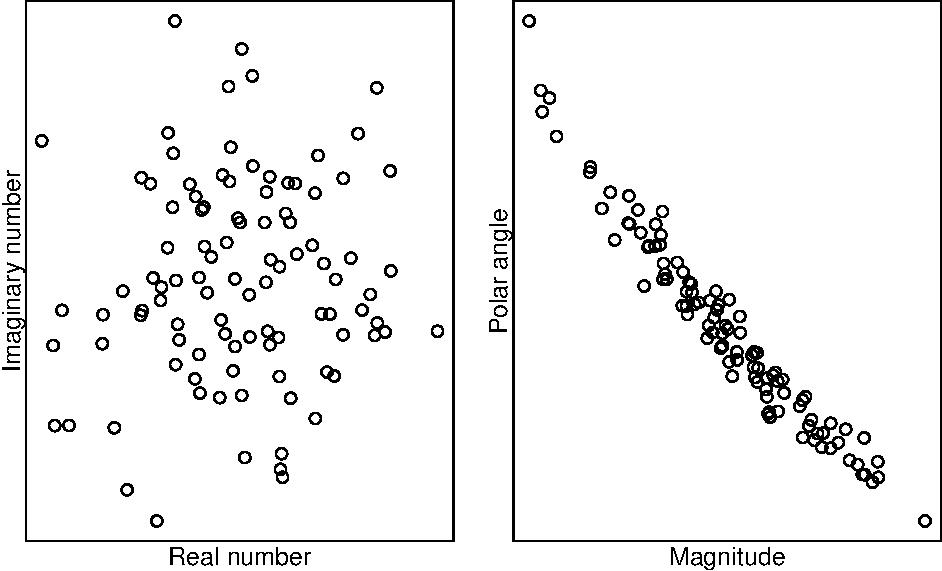
\includegraphics{Svetunkov---Svetunkov---Complex-Dynamic-Models_files/figure-latex/complexCartesianvsPolar-1.pdf}
\caption{\label{fig:complexCartesianvsPolar}Visualisation of complex variables on Cartesian and on polar coordinates planes.}
\end{figure}

In this case, modelling can be done in the exponential form of complex variables, which might allow capturing complicated non-linear relations between variables.

When it comes to operations with complex numbers, mathematically we will say that two complex numbers are equal to each other if and only if their real and imaginary parts are equal:
\begin{equation*}
    \begin{aligned}
        z_1 = & x_1 + i y_1 , \\
        z_2 = & x_2 + i y_2 . \\
        z_1 = & z_2 \iff \left \lbrace
        \begin{aligned}
            & x_1 = x_2 \\
            & y_1 = y_2
        \end{aligned}
        \right. \\
        & \text{ or equivalently } \\
        z_1 = & z_2 \iff \left \lbrace
        \begin{aligned}
            & |z_1| = |z_2| \\
            & \Arg(z_1) = \Arg(z_2)
        \end{aligned}
        \right.
    \end{aligned}
\end{equation*}

Unfortunately, given that complex numbers are two dimensional, it is not possible to say in general whether one variable is greater or less than the other. However, we could use the magnitude to compare complex numbers, to say which one lies further away from the origin than the other. In that case, the variable with a larger magnitude could be considered as a greater than the one with the smaller magnitude. While we could compare the polar angles as well, they only tell us something about the rotation of a complex variable. So, two complex numbers in Figure \ref{fig:complexPlaneCircle} would have the same magnitude, but will have different angles, and it is not possible to say whether one variable is greater than the other in this case -- we would need to devise additional criteria for comparison (e.g.~positive numbers are ``better'' than the negative and/or imaginary ones).

\begin{figure}
\centering
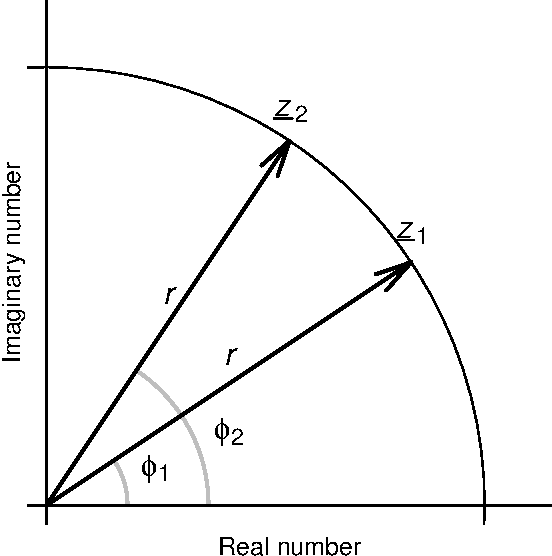
\includegraphics{Svetunkov---Svetunkov---Complex-Dynamic-Models_files/figure-latex/complexPlaneCircle-1.pdf}
\caption{\label{fig:complexPlaneCircle}Comparison of two complex numbers \(z_1\) and \(z_2\) that have the same magnitude \(r\), but different angles.}
\end{figure}

\hypertarget{CLR}{%
\chapter{Complex Linear Regression}\label{CLR}}

\hypertarget{simple-clr}{%
\section{Simple CLR}\label{simple-clr}}

\hypertarget{model-formulation}{%
\subsection{Model formulation}\label{model-formulation}}

The simple Complex Linear Regression can be written as:
\begin{equation}
    y_r + i y_i = a_0 + i a_1 + (b_0 + i b_1) (x_r + i x_i) + \epsilon_r + i \epsilon_i
    \label{eq:SimpleCLR}
\end{equation}
Given that any complex equation can be represented as a system of two equations, this model can be represented as a system of two linear regressions:
\begin{equation}
    \begin{aligned}
        y_r = & a_0 + b_0 x_r - b_1 x_i + \epsilon_r \\
        y_i = & a_1 + b_0 x_i + b_1 x_r + \epsilon_i
    \end{aligned}
    \label{eq:SimpleCLRSystem}
\end{equation}
This model captures a very specific dynamics between the real and imaginary parts, given that they share the same set of parameters for the slope.

\hypertarget{estimation}{%
\subsection{Estimation}\label{estimation}}

Number of estimated parameters is k, number of degrees of freedom per series is k/2.

\hypertarget{inference}{%
\subsection{Inference}\label{inference}}

\hypertarget{forecasting}{%
\subsection{Forecasting}\label{forecasting}}

\hypertarget{multiple-clr}{%
\section{Multiple CLR}\label{multiple-clr}}

\hypertarget{model-formulation-1}{%
\subsection{Model formulation}\label{model-formulation-1}}

\hypertarget{estimation-1}{%
\subsection{Estimation}\label{estimation-1}}

\hypertarget{inference-1}{%
\subsection{Inference}\label{inference-1}}

\hypertarget{forecasting-1}{%
\subsection{Forecasting}\label{forecasting-1}}

  \bibliography{library.bib,packages.bib,websites.bib}

\end{document}
